%=======================================================================================================
% Hyperbolic Grid Generator Documentation
%=======================================================================================================
\documentclass[11pt]{article}
% \usepackage[bookmarks=true]{hyperref}  % this changes the page location !
\usepackage[bookmarks=true,colorlinks=true,linkcolor=blue]{hyperref}

% \input documentationPageSize.tex
\hbadness=10000 
\sloppy \hfuzz=30pt

% \voffset=-.25truein
% \hoffset=-1.25truein
% \setlength{\textwidth}{7in}      % page width
% \setlength{\textheight}{9.5in}    % page height

\usepackage{calc}
\usepackage[lmargin=.75in,rmargin=.75in,tmargin=.75in,bmargin=.75in]{geometry}


\input homeHenshaw


% \input{pstricks}
% \input{pst-node}
% \input{colours}

\usepackage{graphicx}
% \usepackage{epsfig}
% \usepackage{graphics}    
% \usepackage{moreverb}
\usepackage{amsmath}
% \usepackage{fancybox}
% \usepackage{subfigure}

% \usepackage{program} % trouble with pdflatex
\usepackage{algorithm} 
\usepackage{algpseudocode} % algorithmcx 
% \newtheorem{algorithm}{Algorithm}[section] 

% bc = boldCommand
\newcommand{\bc}[1]{\mbox{\bf#1}}   % bold name
\newcommand{\cc}[1]{\mbox{  : #1}}  % comment

\usepackage{makeidx} % index
\makeindex
\newcommand{\Index}[1]{#1\index{#1}}

\usepackage{tikz}
\input trimFig.tex


\input  wdhDefinitions

% Put figures in cgDoc/fig
\newcommand{\figures}{../fig}
% \newcommand{\figures}{\homeHenshaw/OvertureFigures}
\newcommand{\mapping}{\homeHenshaw/Overture/mapping}

% *** See http://www.eng.cam.ac.uk/help/tpl/textprocessing/squeeze.html
% By default, LaTeX doesn't like to fill more than 0.7 of a text page with tables and graphics, nor does it like too many figures per page. This behaviour can be changed by placing lines like the following before \begin{document}

\renewcommand\floatpagefraction{.95}
\renewcommand\topfraction{.95}
\renewcommand\bottomfraction{.95}
\renewcommand\textfraction{.05}   
\setcounter{totalnumber}{50}
\setcounter{topnumber}{50}
\setcounter{bottomnumber}{50}

% ------------------------------------------------------------------------------------------------------------------------------------
% ------------------------------------------------------------------------------------------------------------------------------------
% ------------------------------------------------------------------------------------------------------------------------------------
\begin{document}



\vspace{3\baselineskip}
\begin{flushleft}
  {\Large 
   The Overture Hyperbolic Grid Generator \\
   User Guide, Version 1.0 \\
  }
\vspace{ 2\baselineskip}
William D. Henshaw  \\
Department of Mathematical Sciences, \\
Rensselaer Polytechnic Institute, \\
Troy, NY, USA, 12180. \\
\vspace{2\baselineskip}
\today 
% Centre for Applied Scientific Computing \\
% Lawrence Livermore National Laboratory    \\
% Livermore, CA, 94551   \\
% henshaw@llnl.gov \\
% http://www.llnl.gov/casc/people/henshaw \\
% http://www.llnl.gov/casc/Overture \\
% \vspace{1\baselineskip}
% \today \\
% \vspace{\baselineskip}
% UCRL-MA-134240

\end{flushleft}

\vspace{1\baselineskip}

\begin{abstract}
This document describes the {\ff HyperbolicMapping} class for generating surface
and volume grids using a marching algorithm. Surface grids can be grown over
any other Mapping that defines a surface in three-dimensions including a
{\tt CompositeSurface} which represents a surface as a collection of multiple
sub-surfaces. Volume grids can be generated in two or three space dimensions.
A variety of boundary conditions are available.
\end{abstract}


% \vfill\eject
\tableofcontents


%- 
%- \begin{figure}[hbt]
%- \begin{center}
%-   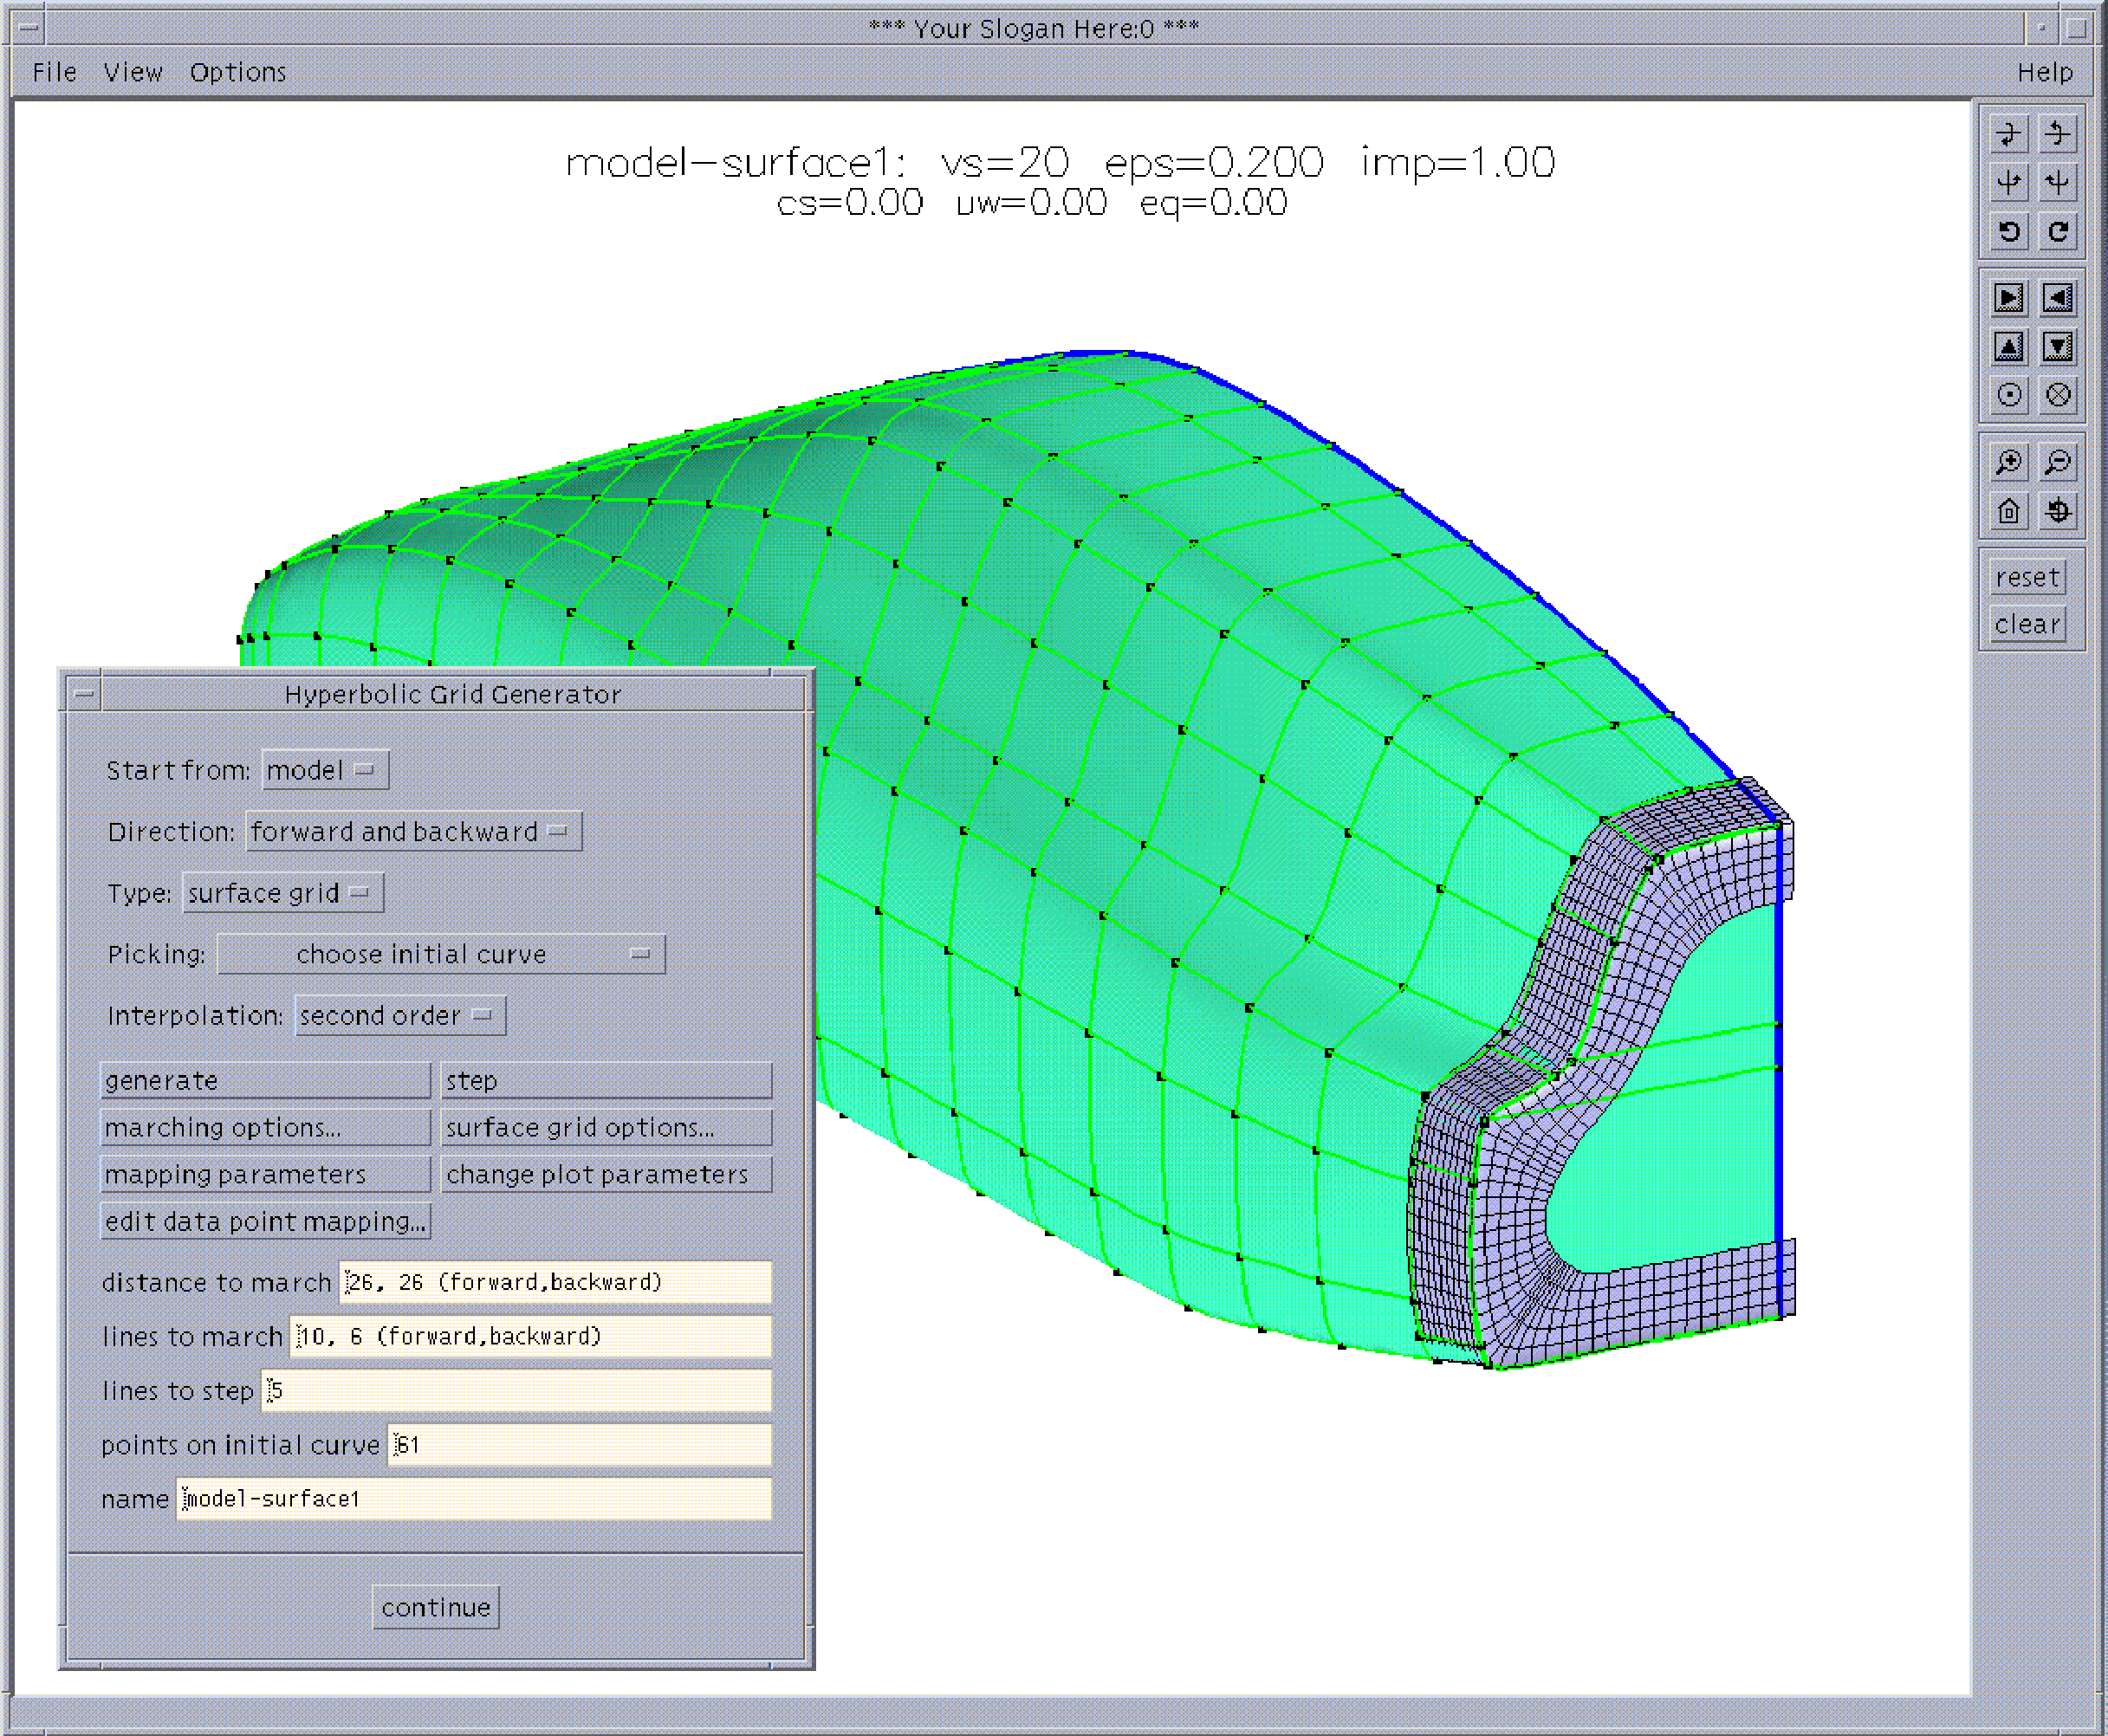
\epsfig{file=\figures/hypeScreen.ps,width=.95\linewidth}  \\
%- \caption{Snapshot of the hyperbolic grid generator. A surface grid is grown on a CAD
%-   model for an automobile. A starting curve is chosen and the grid is grown in both directions
%-    over the surface.}
%-   \end{center} 
%-   \label{fig:screenAsmo}
%- \end{figure}

\clearpage
\input HyperbolicMapping

\vfill\eject
\bibliography{\homeHenshaw/papers/common/henshaw,\homeHenshaw/papers/common/henshawPapers}
\bibliographystyle{siam}

\printindex

\end{document}
